\begin{figure*}[t]
  \centering
  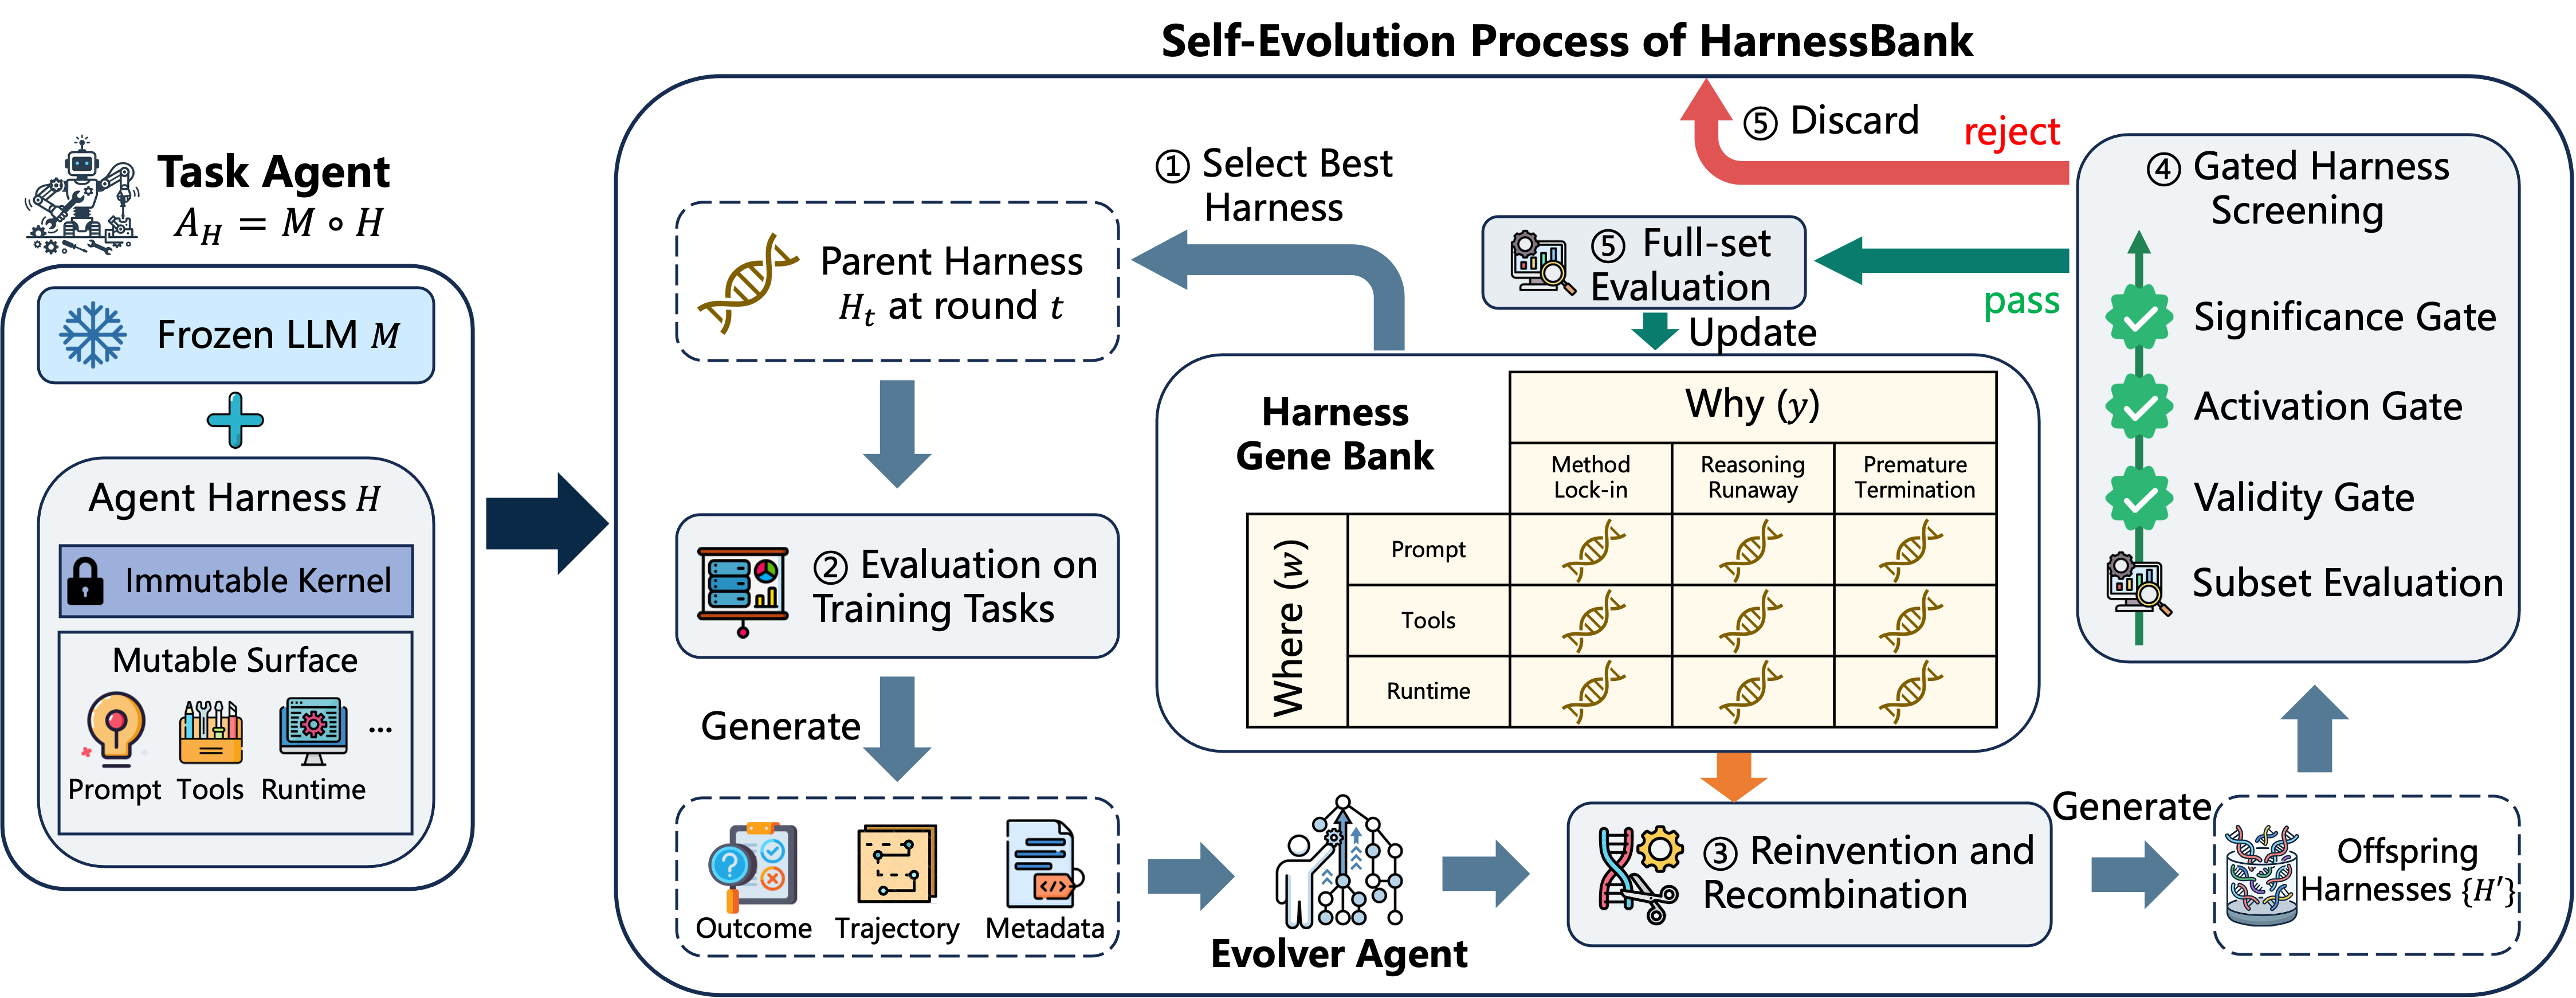
\includegraphics[width=0.9\textwidth]{figures/framework.png}
  \caption{The framework of HarnessBank: 1) The best harness at round $t$ is selected; 2) The comprehensive diagnosis on training tasks is obtained; 3) The offspring harnesses are reinvented or recombined based on Harness Gene Bank; 4) High-quality harnesses are filtered by Gated Harness Screening; 5) Passed harnesses are evaluated and inserted into bank cells according to the principle of competitive selection.}
  \label{fig:loop}
\end{figure*}

\section{Method}
\label{sec:method}

As illustrated in Figure~\ref{fig:loop}, HarnessBank evolves the harness of a task agent through an iterative procedure.
%

\subsection{Problem Formulation}

\paragraph{Agent harness and mutable surface.}
Let $M$ denote a frozen LLM and $H$ its surrounding agent harness, including prompts, injected knowledge, tool specifications, runtime control logic, recovery mechanisms, and configurations.
%
The resulting task agent is:
\begin{equation}
A_H = M \circ H.
\end{equation}
%
Agent-harness self-evolution keeps the weights of $M$ fixed and modifies only $H$.
%
To preserve valid comparison, we partition the harness into an immutable kernel $\mathcal{K}$ and a mutable surface $\mathcal{X}$:
\begin{equation}
H=\mathcal{K}\cup\mathcal{X},
\quad
\mathcal{K}\cap\mathcal{X}=\varnothing.
\end{equation}
%
The kernel may contains evaluation, bookkeeping, self-evolution, and interface-critical code, whereas $\mathcal{X}$ contains the components that can be optimized.

\paragraph{Optimization objective.}
Let $\mathcal{D}_{\mathrm{tr}}$ denote the training tasks available during evolution and $\mathcal{D}_{\mathrm{te}}$ a test set withheld from all evolution decisions.
%
For task $i$, attempt $k$, and harness $H$, let $s_{i,k}(H)\in[0,1]$ be the task score.
%
We define the average utility score:
\begin{equation}
U(H;\mathcal{D})
=
\frac{1}{|\mathcal{D}|}
\sum_{i\in\mathcal{D}}
\frac{1}{K}
\sum_{k=1}^{K}s_{i,k}(H).
\end{equation}
%
Harness evolution searches for:
\begin{equation}
H^{*}
=
\argmax_{H\in\mathcal{H}(\mathcal{X})}
U(H;\mathcal{D}_{\mathrm{tr}}),
\end{equation}
where $\mathcal{H}(\mathcal{X})$ is the set of harnesses reachable through valid modifications to $\mathcal{X}$.
%
The test set is used only after evolution to assess the train-selected harness.


\subsection{Self-Evolution Based on Harness Gene Bank}
\label{sec:se}
HarnessBank separates four key components.
%
The \emph{task agent} executes tasks under the current harness. The \emph{evolver agent} diagnoses failures and proposes patches. The deterministic \emph{evaluator} controls sampling, scoring, activation logging, and statistical tests. The \emph{harness gene bank} preserves high-performing harnesses across semantic cells.

Conventional greedy evolution may collapse onto a narrow class of safe edits or over-specialize patches to individual training tasks.
%
To address this challenge, we introduce \emph{Harness Gene Bank} (HGB), which preserves high-performing candidate harnesses for iterative reinvention and recombination. HGB is inspired by the quality-diversity principle of MAP-Elites~\citep{mouret2015illuminating}.
%
Unlike conventional MAP-Elites, HGB uses semantic pathology descriptors, admits only verified candidates, and prioritizes the strongest lineage under a limited rollout budget.

\paragraph{Semantic cells.}
At round $t$, HGB maintains a categorical bank
\begin{equation}
\mathcal{A}_t:
\mathcal{W}\times\mathcal{Y}
\rightarrow
\mathcal{H}(\mathcal{X})\cup\{\varnothing\},
\end{equation}
where $\mathcal{H}(\mathcal{X})$ denotes the set of valid harnesses, and each cell
$c=(w,y)$ corresponds to a preserved harness.
%
Here, $w$ specifies \emph{where} it acts, and $y$ specifies \emph{why} it is introduced.
%
The \where{} coordinate belongs to:
\begin{equation}
\mathcal{W}
=
{
\texttt{prompt},
\texttt{knowledge},
\texttt{runtime},
\texttt{config}
},
\end{equation}
which is determined from the modified component.
%
The \why{} coordinate belongs to an evolving pathology set $\mathcal{Y}$ and is inferred from failure trajectories.
%
%For simplification, we denote the semantic descriptor $d(H)=\bigl(w,y(p)\bigr)$
%
For example, a selective recovery mechanism for reasoning-budget exhaustion occupies
$(\texttt{runtime},\texttt{thinking-runaway})$.
%
%The information from cells guides the generation of evolved harnesses.
%
At initialization, the gene bank is blank and $\mathcal{A}_0(c)=\varnothing$ for any $c$.
%

Harness indexes harnesses by targeted pathology rather than task-identity biases to search for reusable corrections.
%
Harnesses addressing the same hypothesized mechanism compete within one cell and only the best one is preserved, whereas harnesses targeting different pathologies remain available for recombination.
%
HGB preserves diverse, organized, and high-quality harnesses, which effectively expand the exploration space of offspring harness generation described in the following.


\paragraph{Heredity and variation.}
At round $t$, let $H_t$ denote the currently best harness sampled from the vanilla harness and the harness gene bank according to the quality-biased selection rule:
%
\begin{equation}
H_t
=
\argmax_{H \in
\left(\{H_0\}\cup\operatorname{Im}(\mathcal{A}_t)\right)
\setminus\{\varnothing\}}
U\!\left(H;\mathcal{D}_{\mathrm{tr}}\right).
\label{eq:bst}
\end{equation}
%
where $\operatorname{Im}(\mathcal{A}_t)$ is the image of $\mathcal{A}_t$, i.e., the set of all available harnesses in HGB.
%
$H_t$ serves as the parent harness in this round and has been evaluated on $\mathcal{D}_{\mathrm{tr}}$ while entering the bank.
%
For each training task, we have its outcome $s_{i,k}(H_t)$, trajectory $\tau_{i,k}(H_t)$, and evaluation metadata $e_{i,k}(H_t)$, forming a comprehensive diagnosis:
%
\begin{equation}
\mathcal{L}(H_t;\mathcal{D}_{\mathrm{tr}})
=
\left\{
\bigl(
s_{i,k}(H_t),
\tau_{i,k}(H_t),
e_{i,k}(H_t)
\bigr)
\right\}_{i\in\mathcal{D}_{\mathrm{tr}},\,k\in[K]}.
\label{eq:diag}
\end{equation}
%
Based on the diagnosis $\mathcal{L}(H_t;\mathcal{D}_{\mathrm{tr}})$ and the whole HGB, the evolver agent generates a batch of offspring harnesses $\{H'\}$ with a set $\{(w',y')\}$ indicating \emph{where} and \emph{why} these harnesses are evolved. Each new harness may be either newly invented or a combination of compatible harnesses from different bank cells.
%
For convenience, we denote the semantic descriptor $(w',y')$ of the harness $H'$ as $d(H')$.

\paragraph{Evolved harness selection.}
Given a batch of evolved harnesses, we need to find harnesses that actually improve upon the parent harness $H_t$.
%
Since inspecting and evaluating numerous harnesses on $\mathcal{D}_{\mathrm{tr}}$ is costly, we propose Gated Harness Screening to efficiently filter $N$ harnesses $B=\{H'_j\}_{j=1}^N$ likely to perform better than $H_t$, which will be introduced in detail in Section \ref{sec:vca}.
%
We evaluate every filtered harness $H'_j$ on the whole $\mathcal{D}_{\mathrm{tr}}$ and update its corresponding cells by the principle of competitive selection:
\begin{equation}
\mathcal{A}_{t+1}(d(H'_j))
=
\begin{cases}
H'_j,
&
\mathcal{A}_{t}(d(p)) = \varnothing,
\\[1.5mm]
H'_j,
&
U(H'_j;\mathcal{D}_{\mathrm{tr}})
>
U(\mathcal{A}_{t}(d(p));\mathcal{D}_{\mathrm{tr}}),
\\[1.5mm]
\mathcal{A}_{t}(d(p)),
&
\text{otherwise}.
\end{cases}
\label{eq:archive-update}
\end{equation}
%
Archive admission supports continued exploration but does not constitute final held-out credit.

The self-evolution of harnesses terminates after at most $R$ rounds or after $P$ consecutive rounds without a cell update.
%
Finally, the best harness is selected by Eq. \ref{eq:bst} and evaluated on the test tasks $\mathcal{D}_{\mathrm{te}}$.
%
We note that the test set is never used in the harness self-evolution.
%
%The complete algorithm and implementation details are provided in Supplementary Material.

\subsection{Gated Harness Screening}
\label{sec:vca}
The offspring harnesses $\{H'\}$ at round $t$ may contain various defects and may not improve upon the parent harness $H_t$.
%
However, evaluating all of $\{H'\}$ on the whole training set $\mathcal{D}_{\mathrm{tr}}$ is costly.
%
Therefore, we propose Gated Harness Screening, which efficiently evaluates $\{H'\}$ on a randomly sampled subset $\mathcal{D}_{\mathrm{sub}}$ of $\mathcal{D}_{\mathrm{tr}}$, and integrates three logic gates to mitigate the subset bias and filter out defective harnesses.
%
The computation of these gates is based on a comprehensive diagnosis on $\mathcal{D}_{\mathrm{sub}}$, defined in Eq. \ref{eq:diag}.

\paragraph{Validity and activation gates.}
The validity gate ensures that evaluation outcomes are obtained under a functioning evaluation environment.
%
Infrastructure failures, such as sandbox crashes or verifier timeouts, trigger a predefined repair-and-retry procedure rather than being immediately counted as agent failures.
%
A candidate $H'$ passes when its evaluation produces a complete protocol-valid ledger:
\begin{equation}
g_{\mathrm{valid}}(H';\mathcal{D}_{\mathrm{sub}})
=
\mathbb{I}
\left[
\mathcal{L}(H';\mathcal{D}_{\mathrm{sub}})
\text{ is protocol-valid}
\right].
\end{equation}

The activation gate verifies that the proposed mechanism actually executes.
%
The increment of each candidate harness (i.e., harness patches in $H'$ and not in $H_0$) declares an activation specification and emits a deterministic beacon when triggered.
%
Let $b_{i,k}(H')\in\{0,1\}$ indicate whether the increment of $H'$ activates on task $i$ and attempt $k$.
%
Then
\begin{equation}
g_{\mathrm{act}}(H';\mathcal{D}_{\mathrm{sub}})
=
\mathbb{I}
\left[
\sum_{i=1}^{|\mathcal{D}_{\mathrm{sub}}|}
\sum_{k=1}^{K}b_{i,k}(H')>0
\right].
\end{equation}
%
An evolved but never-triggered harness is treated as inert.
%
%Recombined patches retain independent activation beacons and are evaluated as a new candidate.

\paragraph{Significance gate.}
HarnessBank compares candidate and parent harnesses on identity tasks.
%
For the candidate $H'$, the task-level paired difference of the $i$th training task and total $K$ attempts is defined as:
\begin{equation}
\delta_i
=
\frac{1}{K}
\sum_{k=1}^{K}
\left[
s_{i,k}(H')-s_{i,k}(H_{\mathrm{t}})
\right].
\end{equation}
%
For training tasks, the estimated improvement and paired statistic are
\begin{equation}
\widehat{\Delta}
=
\frac{1}{|\mathcal{D}_{\mathrm{sub}}|}\sum_{i=1}^{|\mathcal{D}_{\mathrm{sub}}|}\delta_i,
\qquad
z
=
\frac{\widehat{\Delta}}
{\widehat{\sigma}_{\delta}/\sqrt{|\mathcal{D}_{\mathrm{sub}}|}},
\end{equation}
where $\widehat{\sigma}_{\delta}$ is the sample standard deviation of the paired differences.
%
The significance gate indicates whether the improvement is significant:
\begin{equation}
g_{\mathrm{sig}}(H';\mathcal{D}_{\mathrm{sub}})
=
\mathbb{I}
\left[\widehat{\Delta}>0
\right]
\times
\mathbb{I}
\left[z\geq1.96
\right]
.
\end{equation}
%
Here, $1.96$ is the $97.5$th percentile of the standard normal distribution, corresponding to the conventional two-sided $5\%$ significance level.
%
Therefore, the paired significance gate removes between-task difficulty variance and makes the decision independently auditable.
%
% Moreover, we use a gain gate to verify whether the modified harness improves upon the parent harness, as follows:
% \begin{equation}
% g_{\mathrm{imp}}(H';\mathcal{D}_{\mathrm{sub}})
% =
% \mathbb{I}
% \left[
% U\bigl(H';\mathcal{D}_{\mathrm{sub}}\bigr)
% >
% U\bigl(H_t;\mathcal{D}_{\mathrm{sub}}\bigr)
% \right]
% .
% \end{equation}

\paragraph{Harness screening.}
Finally, we compute the integrated screening gate $g_{\mathrm{scn}}$ as follows:
\begin{equation}
\begin{aligned}
&g_{\mathrm{scn}}(H';\mathcal{D}_{\mathrm{tr}})\\
=
&g_{\mathrm{valid}}
\bigl(H';\mathcal{D}_{\mathrm{tr}}\bigr)
\times
g_{\mathrm{act}}
\bigl(H';\mathcal{D}_{\mathrm{tr}}\bigr)
\times
g_{\mathrm{sig}}\bigl(H';\mathcal{D}_{\mathrm{tr}}\bigr)
\label{eq:navigation}
\end{aligned}
\end{equation}
%
To improve efficiency, we sequentially compute the value $g_{\mathrm{scn}}$ of each candidate $H'$ and select the first-$N$ passed harnesses.
%
These filtered harnesses further enter the evolved harness selection for a rigorous evaluation, as introduced in Section \ref{sec:se}.
